\documentclass[hidelinks,a4paper,12pt, nofootinbib]{article}
\usepackage[width=15.5cm, left=3cm, top=2.5cm, right=2cm, left=2cm, height= 24.5cm]{geometry}
\usepackage[spanish, es-tabla]{babel} %es-tabla es para que ponga Tabla en vez de Cuadro en el caption
\usepackage[utf8]{inputenc}
\usepackage[T1]{fontenc}
\usepackage{xspace}
\usepackage{xargs}
\usepackage{fancyhdr}
\usepackage{lastpage}
\usepackage{caratula}
\usepackage[bottom]{footmisc}
\usepackage{amsmath}
\usepackage{amssymb}
\usepackage{algorithm}
\usepackage[noend]{algpseudocode}
\usepackage{array}
\usepackage{xcolor,colortbl}
\usepackage{amsthm}
\usepackage{listings}

\usepackage{pgf}
\usepackage{tikz}
\usetikzlibrary{arrows,automata}

\usepackage{graphicx}
\usepackage{sidecap}
\usepackage{amsmath}
\usepackage{wrapfig}
\usepackage{caption}

\usepackage{hyperref}
\hypersetup{
  colorlinks   = true, %Colours links instead of ugly boxes
  urlcolor     = blue, %Colour for external hyperlinks
  linkcolor    = blue, %Colour of internal links
  citecolor   = red %Colour of citations
}

\usepackage{comment}

\usepackage[
  backend=bibtex,
  style=alphabetic
]{biblatex}
\addbibresource{bibliografia.bib}


\captionsetup[table]{labelsep=space}


\setlength{\parindent}{4em}
\setlength{\parskip}{0.5em}

%Defino colores para las tablas
\definecolor{LightCyan}{rgb}{0.77,0.9,0.9}
\definecolor{Gray}{gray}{0.8}


%%fancyhdr
\pagestyle{fancy}
\thispagestyle{fancy}
\addtolength{\headheight}{1pt}
\lhead{Reconocimiento de Patrones}
\rhead{$1º$ cuatrimestre de 2016}
\cfoot{\thepage\ / \pageref{LastPage}}
\renewcommand{\footrulewidth}{0.4pt}
\renewcommand{\labelitemi}{$\bullet$}

%%caratula
\materia{Reconocimiento de Patrones}
\titulo{Trabajos Prácticos}
%\subtitulo{}
%\grupo{}
\integrante{Arrondo, Brian Ariel}{}{}
\integrante{Benzo, Mariano}{}{}
\integrante{Maddonni, Axel Ezequiel}{200/14}{axel.maddonni@gmail.com}
\fecha{... de ... de 2016}

\usepackage{etoolbox}
\AtBeginEnvironment{tikzpicture}{\shorthandoff{>}\shorthandoff{<}}{}{}

\begin{document}
\maketitle

\tableofcontents
\newpage

\section{TP1}
\documentclass[12pt]{article}
\usepackage[spanish]{babel}
\usepackage{amsmath}
\usepackage{graphicx}
\usepackage[utf8]{inputenc}
\usepackage{float} 
\title{\LaTeX}
\date{}
% Este es un comentario, no será mostrado en el documento final.
\begin{document}

\subsection{Ejercicio 2}
La idea de este ejercicio es hacer seis gaussianas bivariadas a partir de seis medias, calculadas por el estimador de máxima verosimilitud, y un sigma elegido a partir de la consigna. \newline
Para hacer esto primero transformo la imagen phantom en una matriz de ALTOxANCHOx3 (RGB) con el comando $imread$. Luego sumo todas las posiciones X e Y de un color, y las divido por la cantidad de pixeles que son de dicho color. De esta forma queda un vector de longitud dos (mu) conformado por la suma de todas las posiciones X dividido la cantidad de pixeles de ese color, y lo mismo para Y.\newline 
Para clasificar la imagen, recorro pixel por pixel toda la imagen y calculo el valor de las seis gaussianas en esa posición. Luego para escoger el color en un pixel, elijo el que me haya dado la probabilidad mas alta. 
\subsubsection{Resultados e Imágenes}
\begin{figure}[H]
\centering

\includegraphics[width=150mm]{tp1/phantom.png}
\caption{Imágen phantom real (verdad terrestre)}
\end{figure}
\begin{figure}[H]
\centering
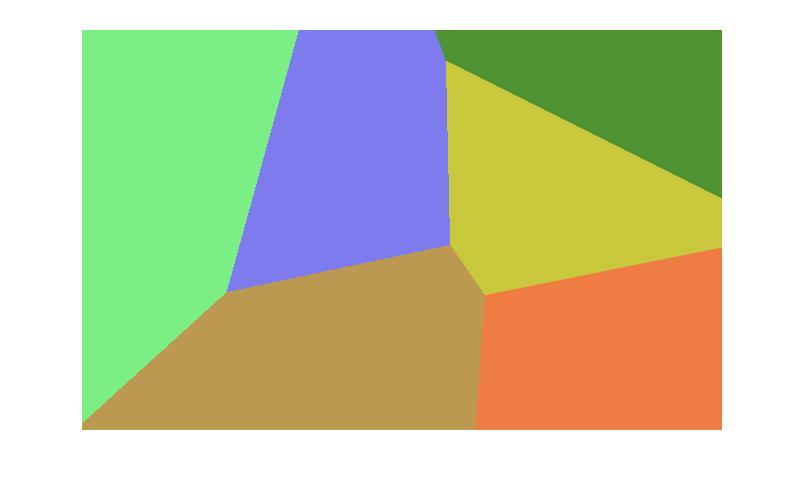
\includegraphics[width=140mm]{tp1/1.jpg}
\caption{Imágen sintética con matrices de covarianza isotrópicas e iguales entre sí}
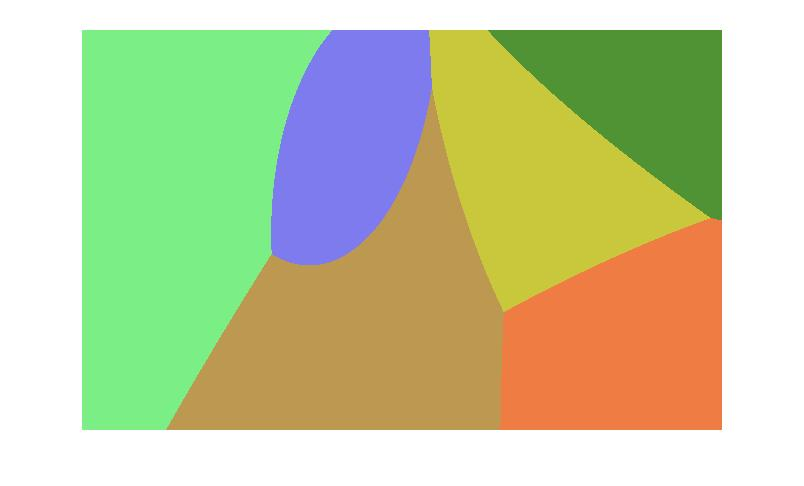
\includegraphics[width=140mm]{tp1/2.jpg}
\caption{Imágen sintética con matrices de covarianza diagonales y diferentes para cada clase}
\end{figure}
\begin{figure}[H]
\centering
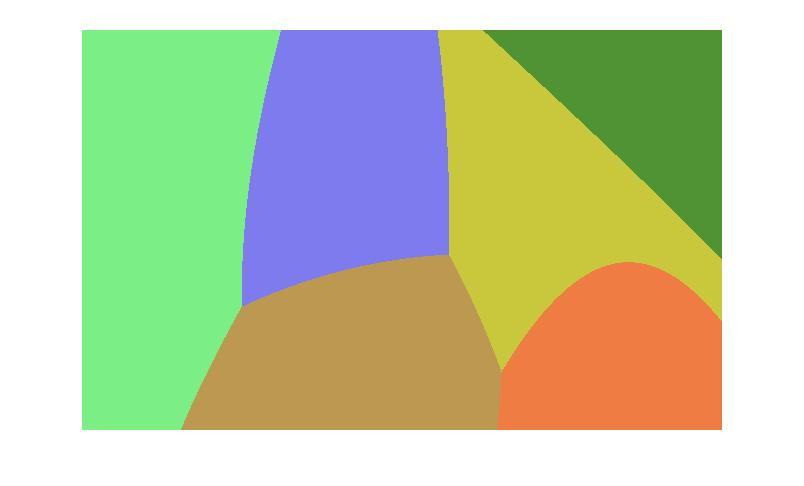
\includegraphics[width=150mm]{tp1/3.jpg}
\caption{Imagen sintética con matrices de covarianza diferentes no-diagonales y diferentes}
 \label{fig:3}
\end{figure}
Para crear las matrices de confusión, creo dos matrices de dos dimensiones ALTOxANCHO (tamaño de la imagen phantom). \newline
\newline
\textbf{Predicciones:}\newline
En la primer matriz recorro pixel por pixel (a la hora de clasificar) colocando números del 1 al 6 en cada posición de esta nueva matriz indicando a que clase pertenece cada pixel (de acuerdo a la clase que haya dado la probabilidad mas alta).\newline\newline
\textbf{Verdad terrestre:}\newline
En la segunda matriz también recorro pixel por pixel y coloco los valores 1,2,3,4,5,6 para indicar a que clase pertenece, y el número 7 para los valores que no pertenecen a ninguna clase de la imagen phantom (no clasificados), ya que en algunas partes de la imagen se pixela y no se puede determinar cuál es la verdadera clase a la que pertenece dicho pixel. \newline
Luego para crear la matriz de confusión uso el comando $confusionmat$ ingresándole dos vectores (primer y segunda matriz apiladas en dos vectores) y un orden (1,2,3,4,5,6,7) con las clases. Las matrices de confusión se muestran al finalizar la compilación de cada archivo del ejercicio 2.\newline\newline
\textbf{Conclusión:}\newline
Se puede observar que, si consideramos la matriz de covarianza igual para cada clase, la separación entre las clases es muy cuadrada. En cambio, se redondea cuando ponemos matrices de covarianza distintas para cada clase. Las imágenes sintéticas no son perfectas, pero se asemejan muy bien a la original en cuanto a posición. \newline
Otro dato interesante es que para que la imagen sintética se acerque a la imagen original phantom se tiene que considerar una matriz de covarianza con valores grandes, ya que, si consideramos valores pequeños, la clasificación es muy estricta y la imagen generada será muy alejada a la original.
\subsection{Ejercicio 3}
En este ejercicio, genero tres Gaussianas trivariadas a partir del estimador de máxima verosimilitud de la media y el sigma (matriz de covarianza). Luego recorro, pixel por pixel, toda la imagen, y calculo la probabilidad de pertenecer a cada clase, con las tres Gaussianas.\newline
Primero transformo la imagen en una matriz de ANCHOxALTOX3 (RGB) con el comando $imread$.\newline 
Para generar las matrices de covarianza, utilizo una función auxiliar $matriz_cov$ que me devuelve el estimador de máxima verosimilitud del sigma, es decir, una matriz cuadrada de 3 dimensiones.\newline\newline 
Para generar las medias (mu) creo un vector de 3 posiciones. En cada posición, primero calculo la suma de todos los elementos de las submatrices ALTOxANCHOx1, ALTOxANCHOx2, ALTOxANCHOx3 (R, G y B) respectivamente. Luego las divido por la cantidad de elementos, y me queda un vector de longitud 3, es decir, el estimador de máxima verosimilitud de la media.\newline\newline
Por ultimo recorro, pixel por pixel, toda la imagen y calculo las probabilidades de que cada pixel pertenezca a cada una de las tres clases, y me quedo con la probabilidad mas alta. Luego lo pinto del color de dicha clase.\newline
 \begin{figure}[H]
\centering
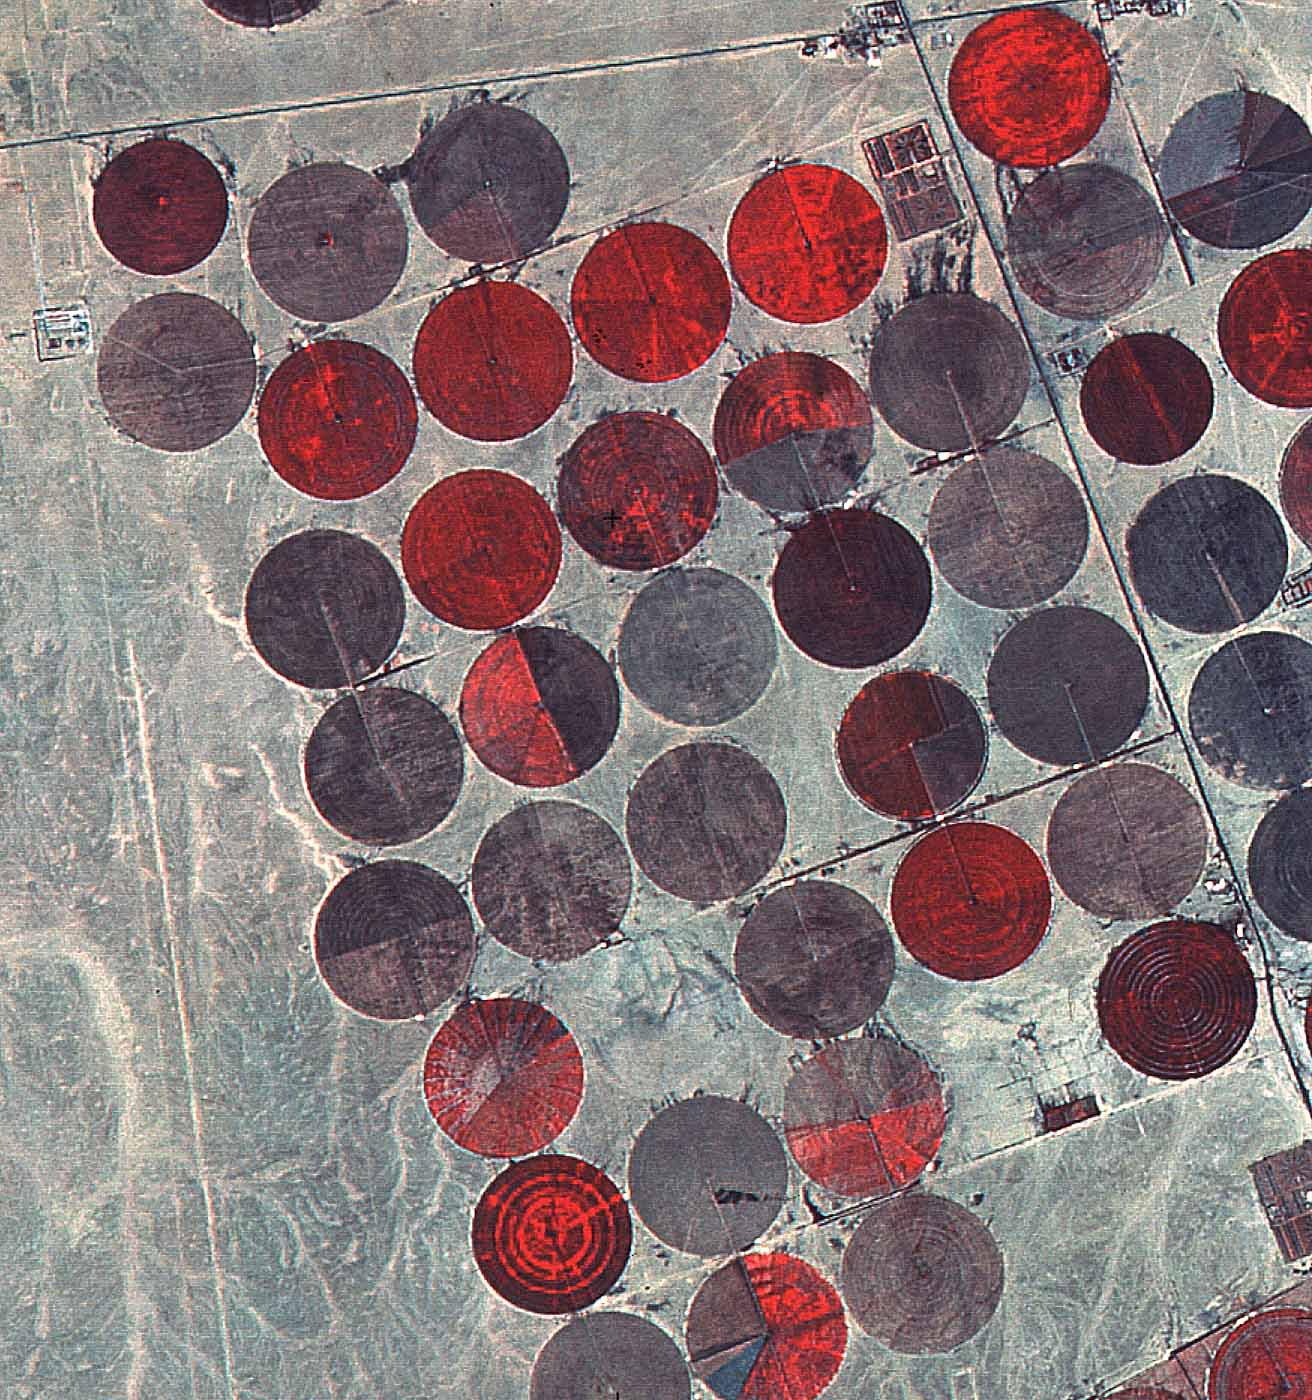
\includegraphics[width=70mm]{tp1/circular.jpg}
\caption{Imágen real}
\includegraphics[width=70mm]{tp1/circular_verdad.png}
\caption{Imágen cultivo verdad terrestre}
\end{figure}
\begin{figure}[H]
\centering
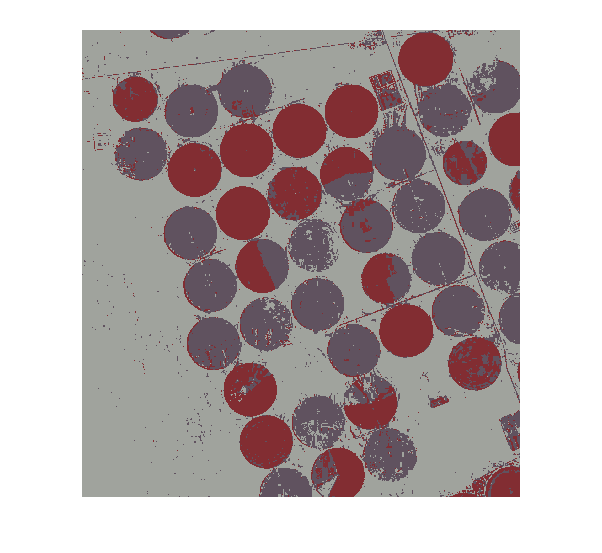
\includegraphics[width=100mm]{tp1/circular_clasificada.png}
\caption{Imágen según clasificación}
\end{figure}
Para hacer la matriz de confusión, con un editor de imágenes creamos una imagen que ofrece la verdad terrestre, es decir, los datos clasificados de manera correcta.\newline 
Para crear la matriz de confusión, creo dos matrices de dos dimensiones ALTOxANCHO (tamaño de la imagen del cultivo).\newline\newline 
\textbf{Predicciones:}\newline
En la primer matriz recorro pixel por pixel (a la hora de clasificar) colocando números del 1 al 3 en cada posición de esta nueva matriz indicando a que clase pertenece cada pixel (de acuerdo a la clase que haya dado la probabilidad mas alta).\newline\newline
\textbf{Verdad terrestre:}\newline
En la segunda matriz también recorro pixel por pixel y coloco los valores 1,2,3 para indicar a que clase pertenece realmente. Luego para crear la matriz de confusión uso el comando confusionmat ingresándole dos vectores (primer y segunda matriz apiladas en dos vectores) y un orden (1,2,3) con las clases. La matriz de confusión se muestra al finalizar la compilación del ejercicio 3.\newline\newline
\textbf{Conclusión:}\newline
Lo interesante de este ejercicio es que la clasificación depende mucho de la selección de las regiones de entrenamiento, ya que a partir de estas se estima la media (Estimador de máxima verosimilitud) y las matrices de covarianza. Si se elige una región de entrenamiento demasiado grande, la clasificación va a ser muy laxa.\newline
Si se elige una región de entrenamiento muy pequeña, la clasificación va a ser muy estricta. Además, influye mucho que sección de la imagen seleccionamos como región de entrenamiento ya que, si tomamos regiones muy similares, se hace muy difícil decidir a qué clase pertenece cada pixel. 

\end{document}
\newpage

\section{TP2}
\input{tp2.tex}
\newpage

\section{TP3: Métodos no-paramétricos}
Los métodos no paramétricos se utilizan para estimar las funciones de densidad de probabilidad (f.d.p.) cuando no se conoce la expresión de la misma ni los parámetros.

\subsection{Esquema general}

Sea una cierta región R del espacio de características. La probabilidad $P_R$ de que un cierto x pertenezca a R viene dada por:

\[ P_R = p(x \in R) = \int_{R} p(x) dx \approx p(x) \int_{R} dx = p(x)*V \]

donde $V$ es el volumen ocupado por la región $R$.

Supongamos que disponemos de N muestras independientes $x_1
, x_2, ..., x_N$ correspondientes a la f.d.p. que queremos estimar, y dados:

\begin{itemize}
\item $k_N$ = cuántas de las N muestras pertenecen a la región R
\item $\frac{k_N}{N}$ es una estimación de $P_R$ para cada x, lo cual es a su vez una estimación de p(x).
\end{itemize}

Usando:
\[ p(x)*V \approx \frac{k_N}{N} \]

Podemos estimar $p(x)$ como :
\[ p(x) = \frac{\frac{k_N}{N}}{V} \]

Es decir, se aproxima $p(x)$ definiendo una región $R$ pequeña alrededor de x y contando cuántos de los $x_i$ caen en $R$.
En los ejercicios se aplicaron dos métodos no paramétricos: 

\begin{itemize}
\item Ventanas de Parzen
\item $k_{n}$ vecinos más cercanos
\end{itemize}

\subsection{Ventanas de Parzen}

Tomando una región $R$ con forma de hipercubo d-dimensional de lado $h_N$, entonces:

\[ V_N = (h_N)^d \]

Y sea la siguiente \textbf{función de ventana}:

\[ \varphi(x) = \left\{
\begin{array}{c l}
  1 & |u_j| \leq \frac{1}{2}, j=1..d \\
  0 & \text{caso contrario}
\end{array}
\right.
\]

Entonces, para un cierto x:

\[ \varphi(\frac{x-x_i}{h_N}) = 1 \text{ si } x_i \in \text{ hipercubo de volumen } V_N \text{ centrado en x} \]

El número de muestras, entonces, se calcula:

\[k_N = \sum_{i=1}^{N} \varphi(\frac{x-x_i}{h_N}) \]

y finalmente podemos estimar la f.d.p. resolviendo:

\begin{equation}
p_N(x) = \frac{\frac{k_N}{N}}{V_N} = \frac{1}{N} \sum_{i=1}^{N} \frac{1}{h_{N}^{d}} \varphi(\frac{x-x_i}{h_N})
\end{equation}

\subsubsection{Pseudocódigo: Ventanas de Parzen}

\begin{algorithm}[H]
  \begin{algorithmic}[1]
  \caption{Pseudocódigo del método de ventanas de parzen}
  \label{algo:3-1}
    \Procedure{parzen\_hipercubo}{$x$ (punto a evaluar), $X$ (muestra), $h$ (tamaño de la ventana), $d$(dimensión)}
	\State $L$ $\gets$ $|X|$
	\State $k_n$ $\gets$ $0$
	\For {$i \in (1..L)$}
		\State $in\_inside$ $\gets$ $0$
		\For {$j \in (1..d)$}
			\If {$|x(j) - X_{i}(j)| / h \leq 0.5$}
				\State $is\_inside++$
			\EndIf
		\EndFor
		\If {$is\_inside == d$}
			\State $k_n++$
		\EndIf
	\EndFor
	\State $p(x)$ $\gets$ $\frac{k_n}{L} / h^d$
	\EndProcedure
	\end{algorithmic}
\end{algorithm}

\subsection{$k_n$ vecinos más cercanos}

A diferencia del método de ventanas de parzen, en este método no se fija el $V_N$ sino que se buscan las $k_N$ muestras más próximas a $x$ y se determina el volumen que las contiene. Es decir, $V_N$ se calcula en función de la muestra. Se estima $p_N$ calculando:

\begin{equation}
p_N(x) = \frac{\frac{k_N}{N}}{V_{k,N}}
\end{equation}

\subsubsection{Pseudocódigo: $k_N$ vecinos más cercanos}

\begin{algorithm}[H]
  \begin{algorithmic}[1]
  \caption{Pseudocódigo del método de $k_N$ vecinos con dimensión 2}
  \label{algo:3-2}
    \Procedure{knn\_2D}{$x$ (punto a evaluar), $X$ (muestra)}
	\State $L$ $\gets$ $|X|$
	\State $k$ $\gets$ $\sqrt{L}$
	\For {$i \in (1..L)$}
		\State $dist(i)$ $\gets$ $||x - X_i||$
	\EndFor
	\State $sort(dist)$
	\State $V$ $\gets$ $\pi * dist(min(L,k))^2$
	\State $p(x)$ $\gets$ $\frac{k}{L} / V$
	\EndProcedure
	\end{algorithmic}
\end{algorithm}

\subsection{Ejercicio 1}

Se realizó un estudio de la convergencia de la f.d.p. de una distribución Gaussiana univariada utilizando el método de Ventanas de Parzen y $k_{n}$ vecinos más cercanos.
Para dicho estudio se implementaron funciones para calcular $N$ iteraciones de la sucesión $p(x)$ evaluada en $x$ = 0, 1 y 2 usando ambos métodos, con $N$ = 10, 100, 1000 y 10000. Para cada valor se usaron muestras de distintos tamaños. (ver código de funciones \texttt{knn\_1D} y \texttt{parzen\_cubo\_1D}.

\subsubsection{Resultados e Imágenes}

\begin{figure}[ht!]
\centering
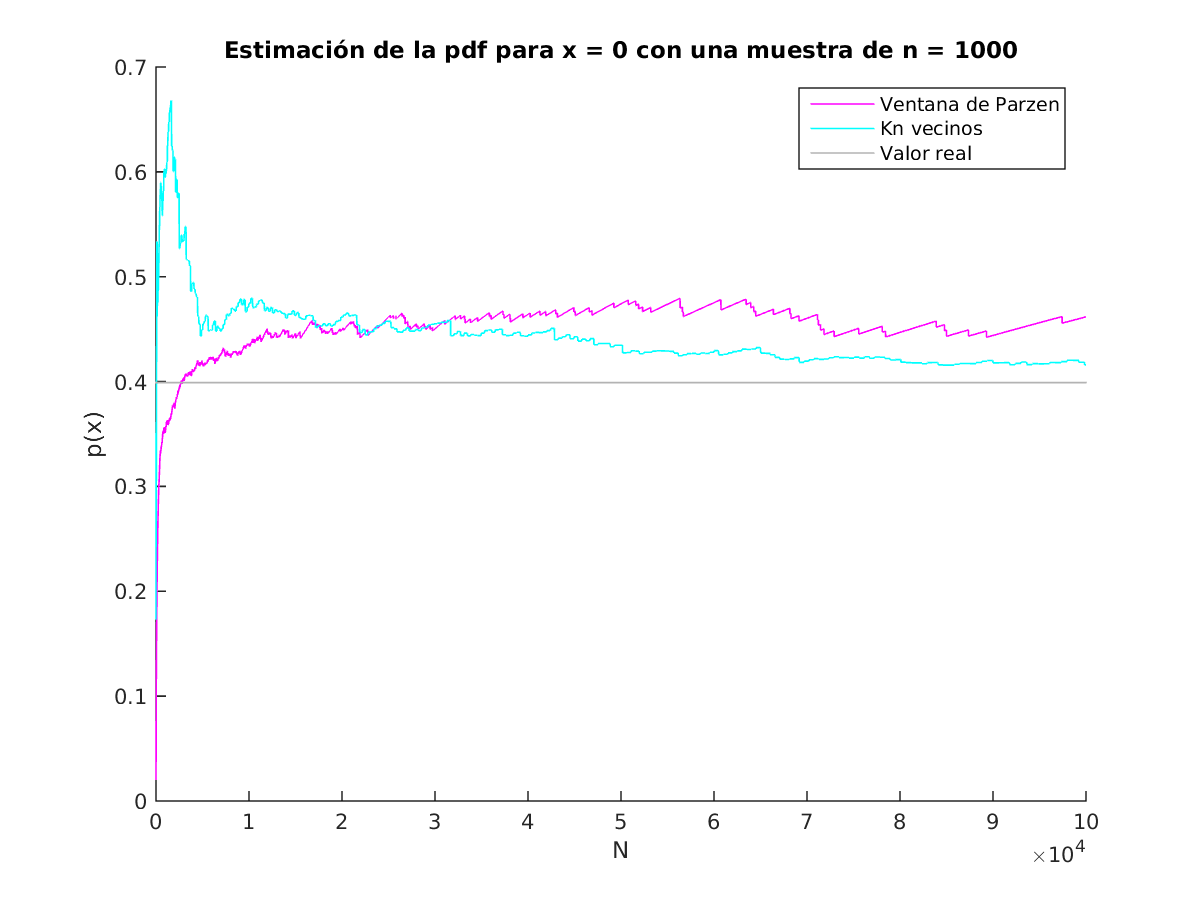
\includegraphics[width=120mm]{img/tp3/ej1-1.png}
\caption{Convergencia de la fdp de una dist. Normal (1,0).}
\end{figure}

\begin{figure}[ht!]
\centering
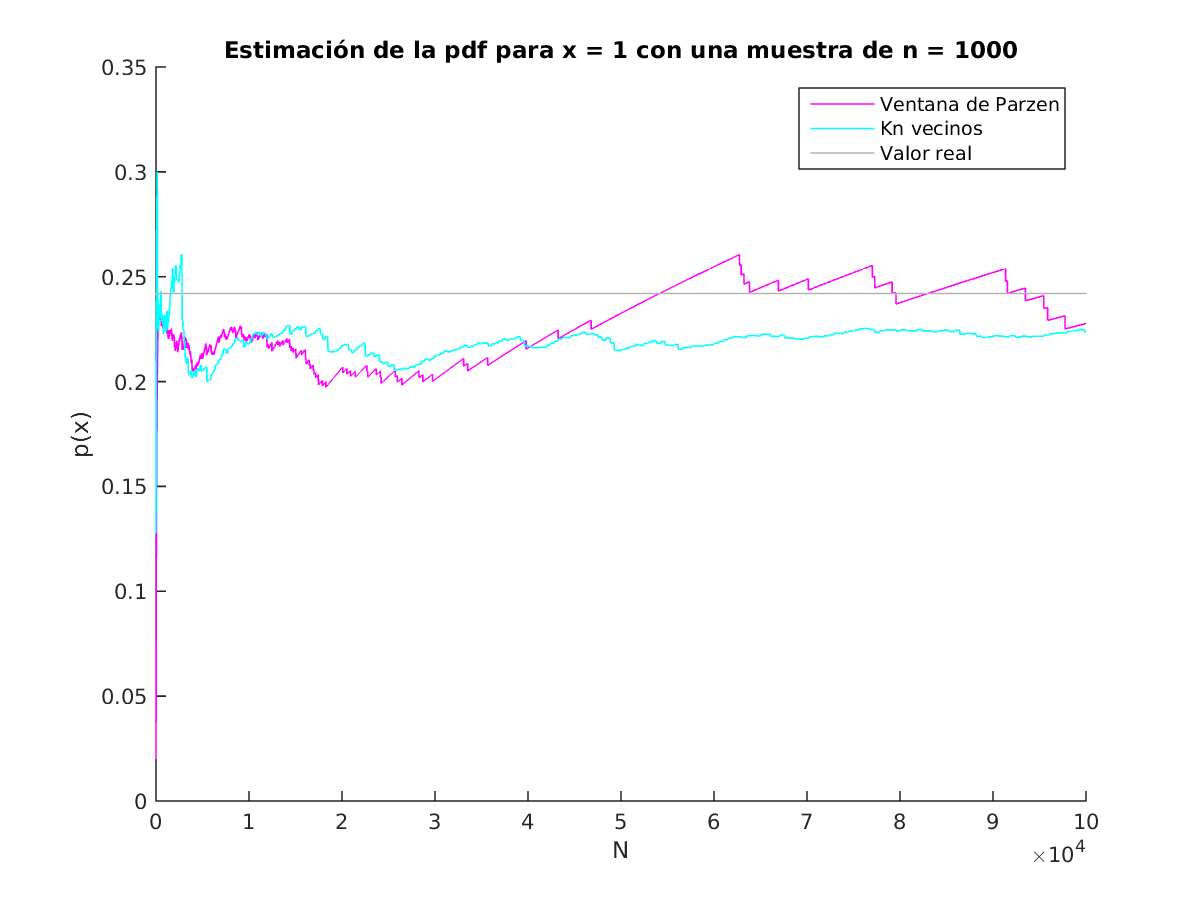
\includegraphics[width=120mm]{img/tp3/ej1-2.png}
\caption{Convergencia de la fdp de una dist. Normal (1,0).}
\end{figure}

\begin{figure}[ht!]
\centering
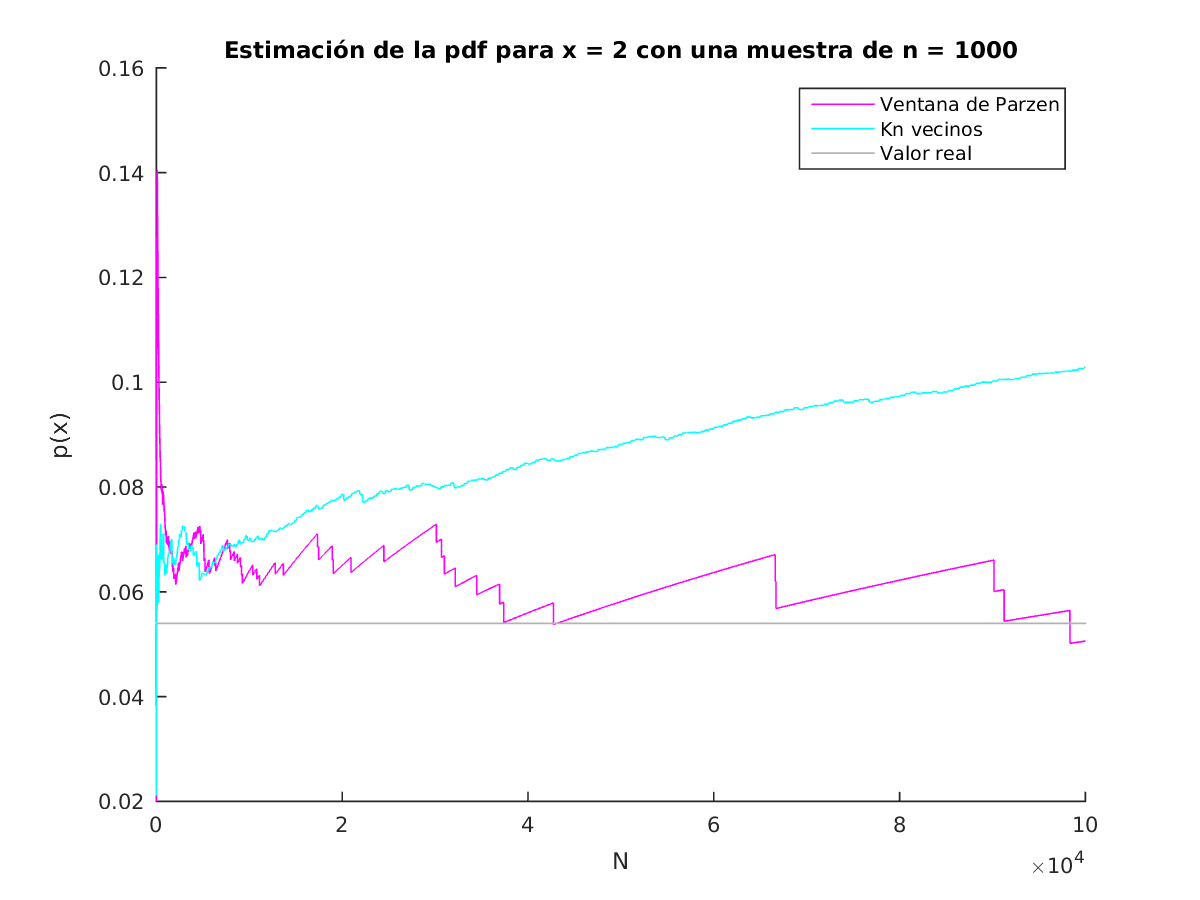
\includegraphics[width=120mm]{img/tp3/ej1-3.png}
\caption{Convergencia de la fdp de una dist. Normal (1,0).}
\end{figure}

\subsection{Ejercicio 2}

En este ejercicio se generaron datos pertenecientes a dos clases $w_1$ y $w_2$, generados a partir de dos Gaussinas bivariadas. Utilizando los métodos mencionados en el ejercicio anterior, adaptados a dos variables, se realizó la partición del espacio de características resultante (dado por las muestras generadas). Para graficar las particiones, se determinaron intervalos bidimensionales rectangulares de tamaño $1x1$ y se evaluaron los centros de cada intervalo para aproximar la $p(x)$ correspondiente ) cada muestra.
A continuación, una comparación de los resultados obtenidos entre los métodos de ventanas de parzen (con un hipercubo de dimensión 2) y $k_nn$ vecinos más cercanos. Además incluimos una comparación usando una ventana circular centrada en el punto a evaluar. Para este último, se implementó un algoritmo de ventanas de Parzen donde el $V$ utilizado es el área del círculo resultante centrado en el $x$ correspondiente, con el radio del círculo ingresado por parámetro. (ver código de función \texttt{parzenr2\_circulo}.

\subsubsection{Resultados e Imágenes}

\begin{figure}
\begin{minipage}{\textwidth}
    \begin{center}
        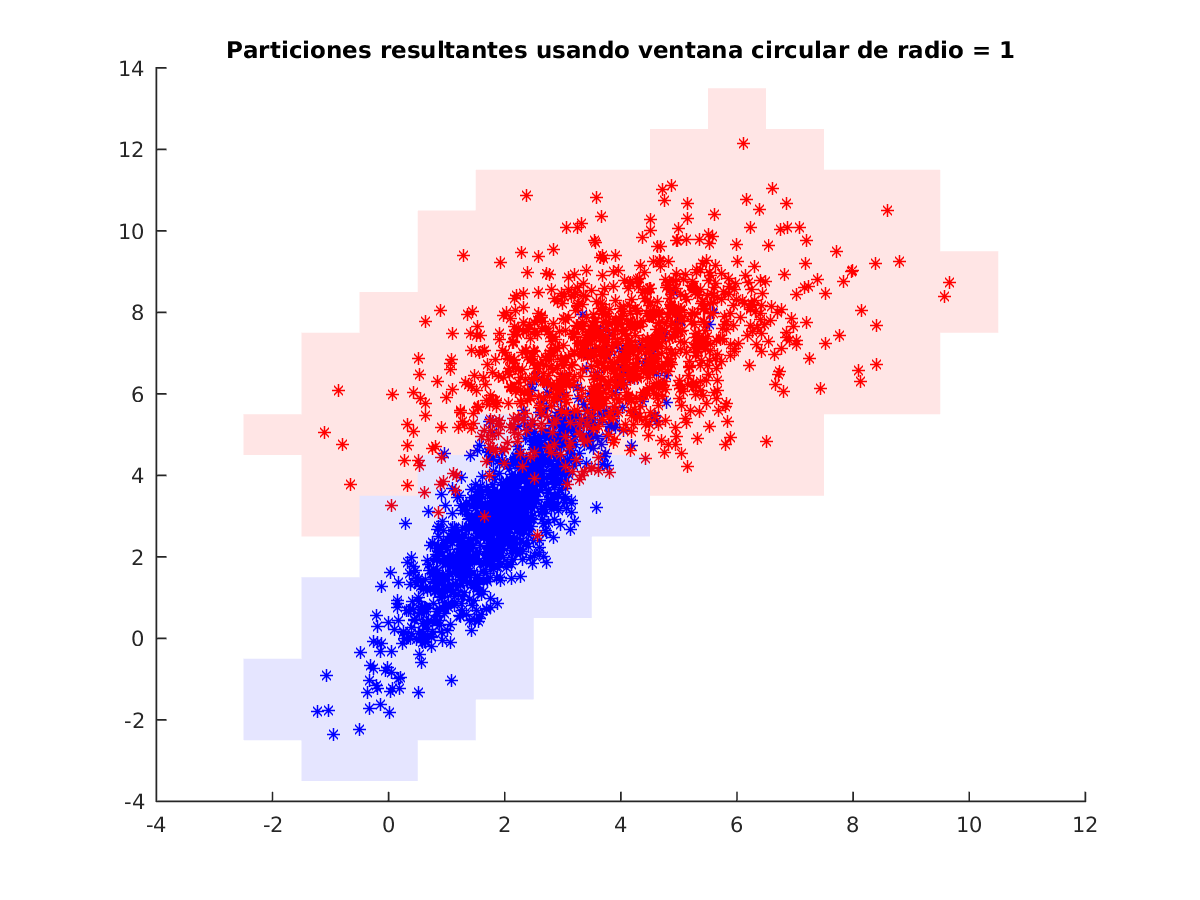
\includegraphics[width=0.4\textwidth]{img/tp3/ej2-1.png}
        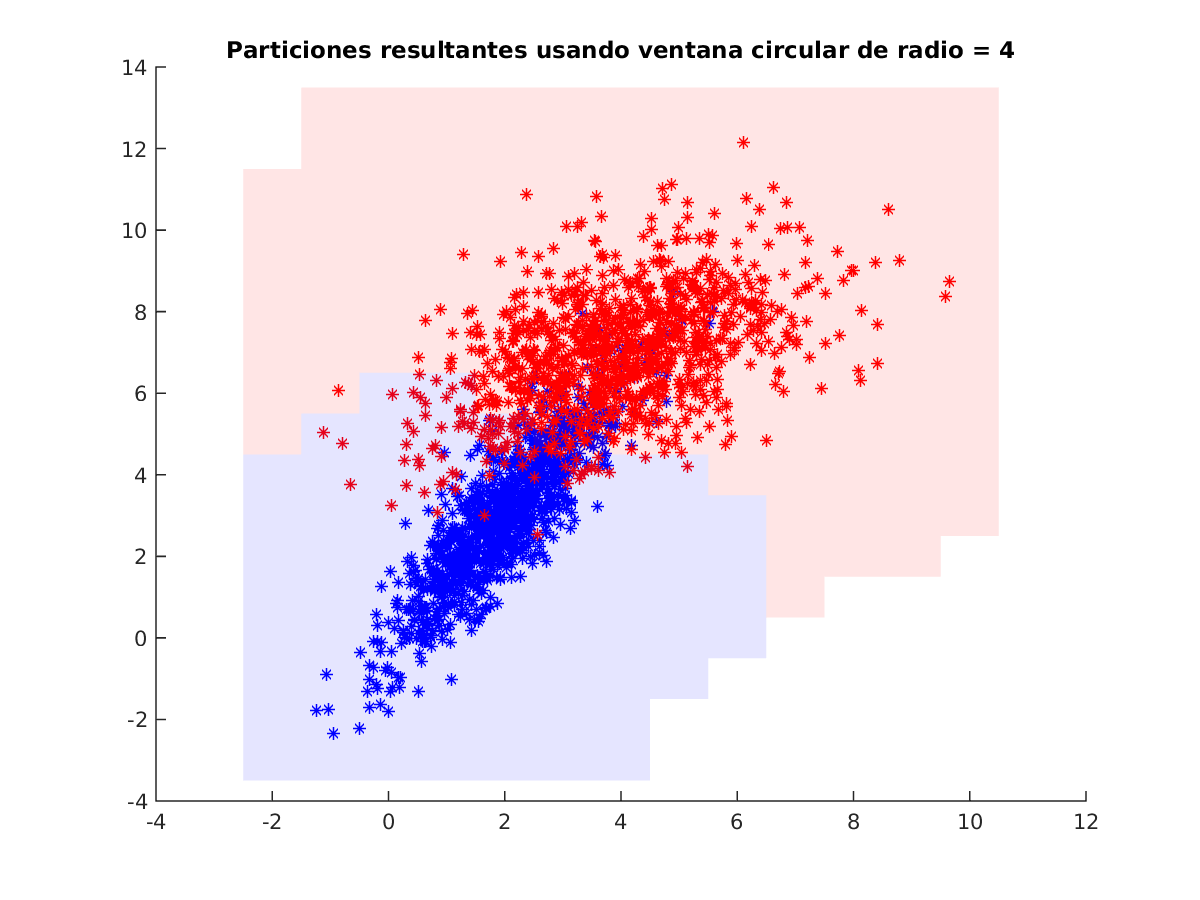
\includegraphics[width=0.4\textwidth]{img/tp3/ej2-3.png}
    \end{center}
\label{minipage:ej2-A}
\end{minipage}
\caption{\footnotesize{División del espacio de características resultante usando ventanas circulares.}} 
\end{figure}

\begin{figure}
\begin{minipage}{\textwidth}
    \begin{center}
        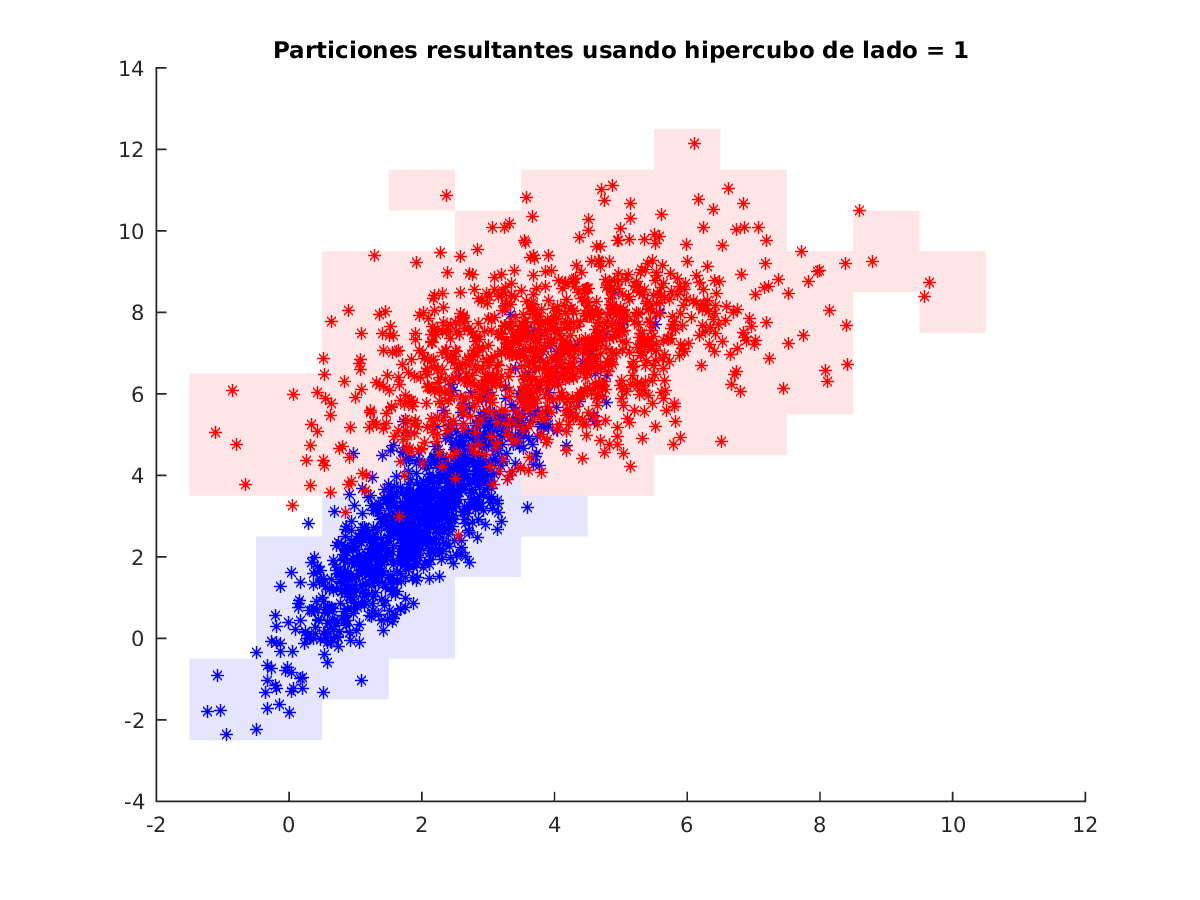
\includegraphics[width=0.4\textwidth]{img/tp3/ej2-2.png}
        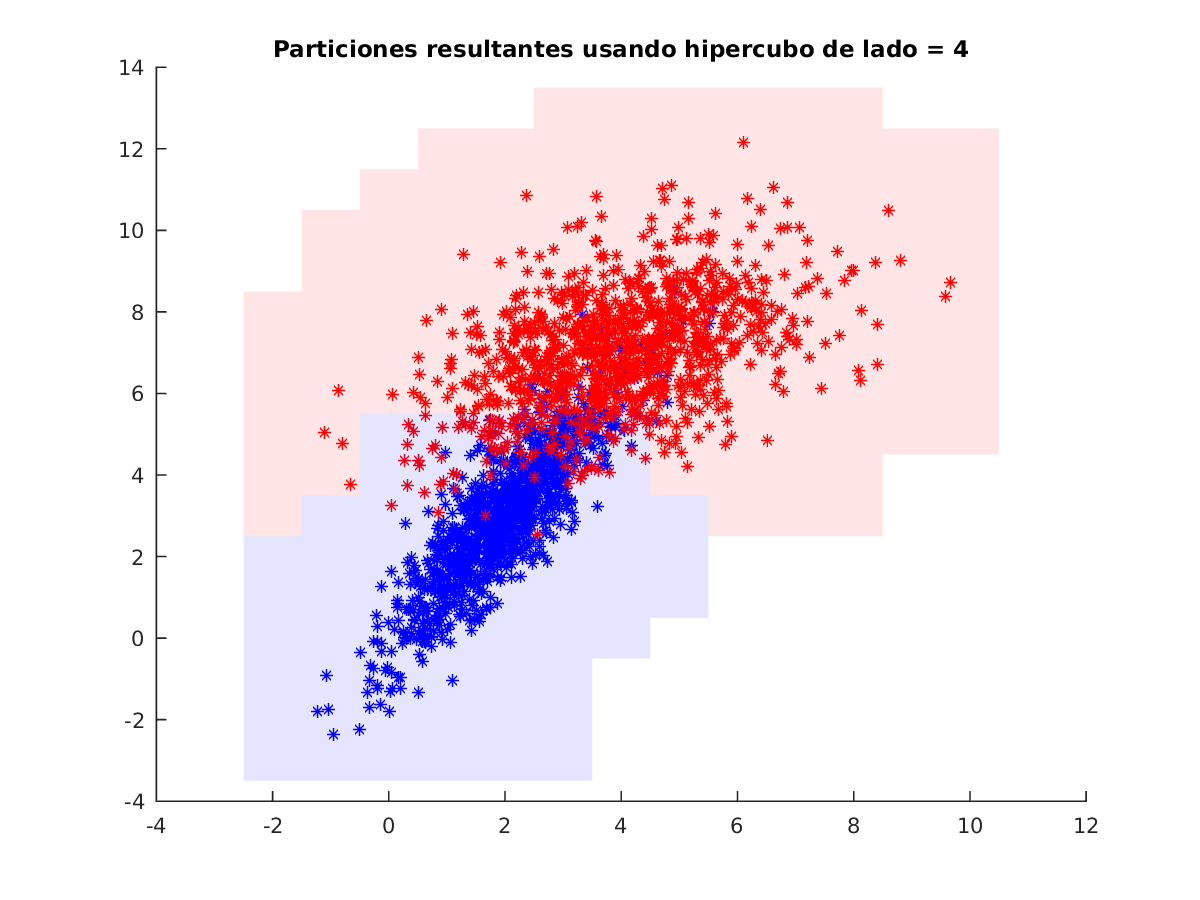
\includegraphics[width=0.4\textwidth]{img/tp3/ej2-4.png}
    \end{center}
\label{minipage:ej2-B}
\end{minipage}
\caption{\footnotesize{División del espacio de características resultante usando ventanas hipercúbicas.}} 
\end{figure}

\begin{figure}[ht!]
\centering
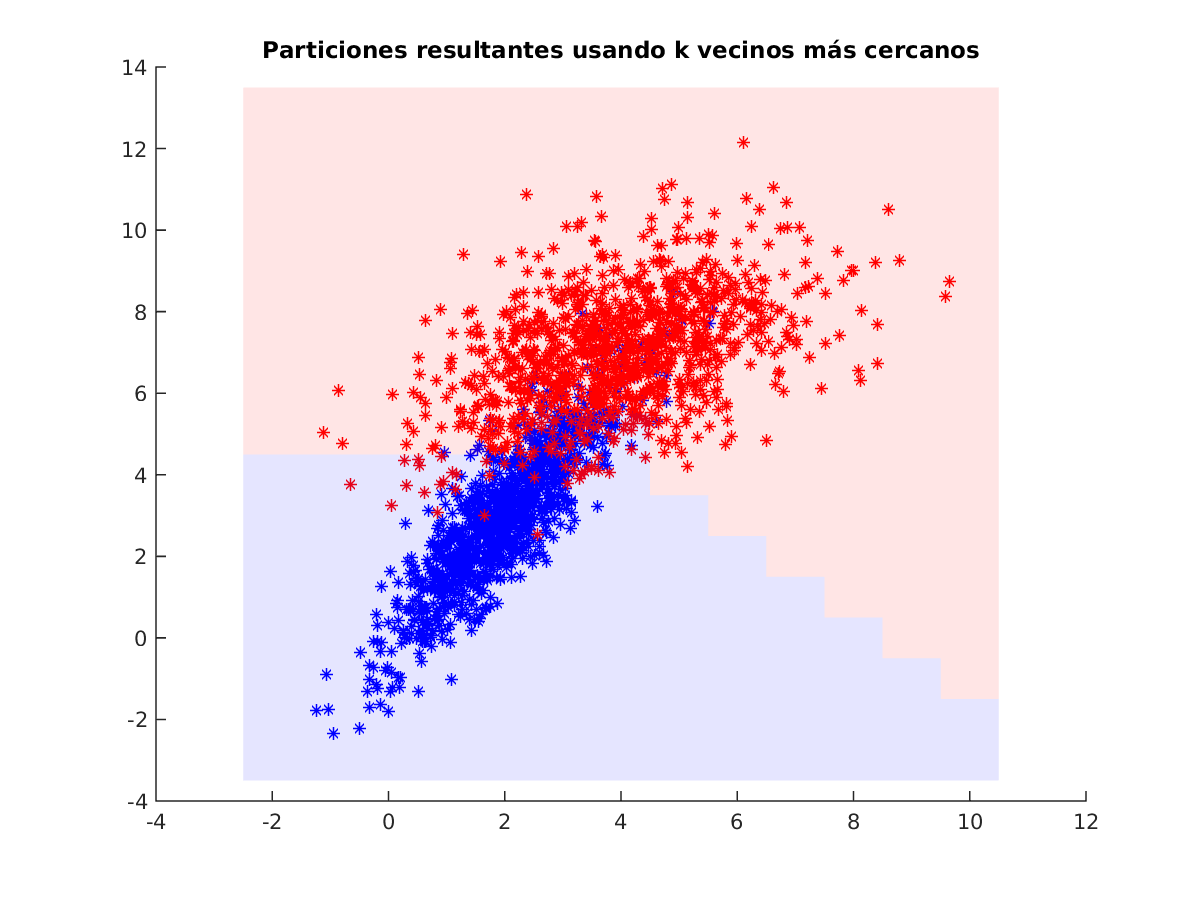
\includegraphics[width=120mm]{img/tp3/ej2-5.png}
\caption{\footnotesize{División del espacio de características resultante usando kvecinos más cercanos.}} 
\end{figure}

Uno de los problemas característicos de este método consiste en encontrar la secuencia de volúmenes $V_i$ o el tamaño de ventana óptimo. Por ejemplo, tomando $V_N$ = $V_1 / N$, los resultados son sensibles a la elección del volumen inicial $V_1$. Si el volumen inicial es muy pequeño, la mayoría de los volúmenes estarán vacíos, y la estimación de $p_n$ se vuelve muy sensible a errores (ver figura ...). Por otro lado, tomando $V_1$ grande, las variaciones en $p(x)$ que caen dentro de la misma ventana se perderán (ver figura ...). Para solucionar este problema, se presenta el siguiente método.

\newpage

\section{TP4: Discriminante de Fisher}
Discriminante lineal de Fisher es un método utilizado en estadística, reconocimiento de patrones y aprendizaje de máquinas para encontrar una combinación lineal de rasgos que caracterizan o separan dos o más clases de objetos o eventos. La combinación resultante puede ser utilizada como un clasificador lineal, o, más comúnmente, para la reducción de dimensiones antes de la posterior clasificación.

\subsection{Ejercicio 1}

Implementación del discriminante lineal de Fisher para 2 clases. En este caso lo que hacemos es buscar el mejor vector posible que maximize la separacion entre las dos clases ingresadas (a este vector lo llamaremos $W$). Luego proyectamos los datos en dicho vector, reduciendo su dimensión de dos a una, lo que facilita la posterior clasificacion.
\\
Uso de la funcion $Fisher(X)$ creada en matlab:\\
Input:
\begin{itemize}
	\item $X$: Matriz de $(NxDxC)$ con los datos a analizar, donde:\\
	\begin{itemize}
	\item	$N$: Cantidad de datos.\\
	\item	$D$: Dimensión de los datos (En este caso 2).\\     
	\item	$C$: Cantidad de clases (En este caso 2).\\
	\end{itemize}
\end{itemize}

\subsubsection{Resultados e Imágenes}

\begin{figure}[ht!]
\centering
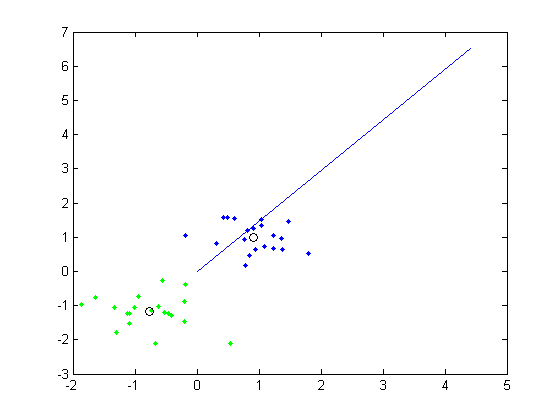
\includegraphics[width=120mm]{img/tp4/ej1-1.png}
\caption{Conjuntos de datos en dos dimensiónes y $W$.}
\end{figure}

\begin{figure}[ht!]
\centering
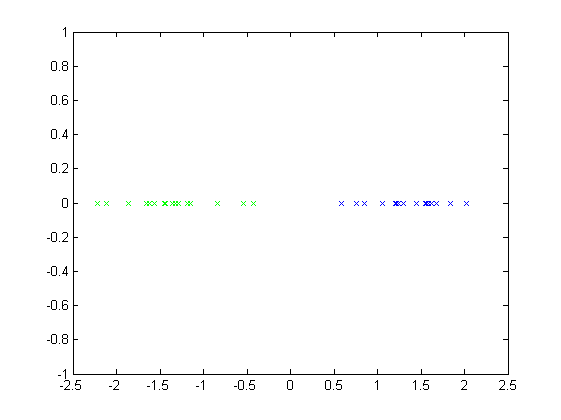
\includegraphics[width=120mm]{img/tp4/ej1-2.png}
\caption{Conjuntos de datos ya proyectados en $W$.}
\end{figure}

\subsection{Ejercicio 2}

Implementación del discriminante lineal de Fisher para 3 o más clases de datos. En este caso, a diferencia del anterior, como los datos de entrada tienen más de dos dimensiónes lo que hacemos es decrementar una a una la dimensión hasta llegar a uno. Otro cambio es el vector $W$ que utilizamos en el punto anterior para proyectar los datos, este ira variando segun la dimensión. Por ejemplo, si se trabaja con datos en tres dimensiónes este vector seria un plano.\\


Uso de la funcion $FDA(X,Y,r)$ creada en matlab:\\

$[Z,W]=FDA(X,Y,r)$\\

Input:
	\begin{itemize}
	\item$X$: Matriz de $(DxN)$ con los datos a analizar, donde:\\
		\begin{itemize}
		\item$D$: Dimensión de los datos.\\
		\item$N$: Cantidad de datos. \\
		\end{itemize}
	\item$Y$: Vector con etiqueta de la clase para cada dato.\\
	\item$r$: Dimensión a la cual queremos llevar nuestros datos.\\
	\end{itemize}
   
Output:
	\begin{itemize}
	\item$W$: $(Dxr)$ matriz de transformación.\\
	\item$Z$: $(rxN)$ matriz con los datos reducida su dimensión.\\
	\end{itemize}
 
\subsubsection{Resultados e Imágenes}

\begin{figure}[ht!]
\centering
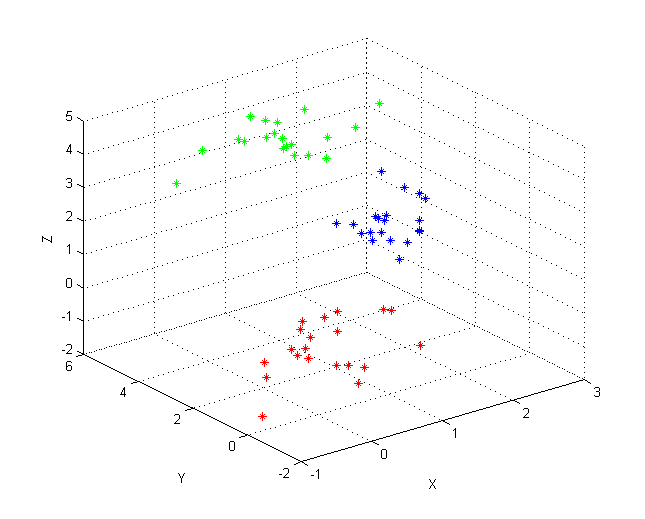
\includegraphics[width=120mm]{img/tp4/ej2-1.png}
\caption{Conjuntos de datos en tres dimensiónes.}
\end{figure}

\begin{figure}[ht!]
\centering
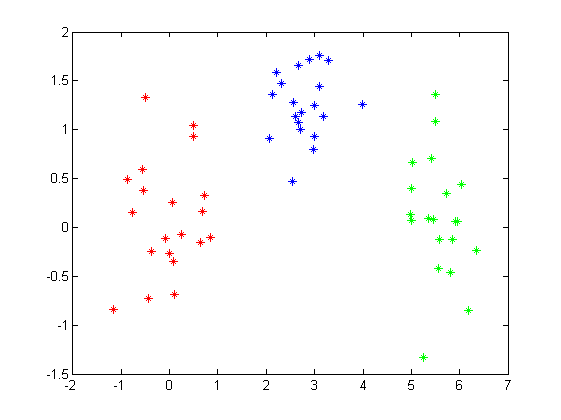
\includegraphics[width=120mm]{img/tp4/ej2-2.png}
\caption{Conjuntos de datos proyectados en $W$(plano).}
\end{figure}

\begin{figure}[ht!]
\centering
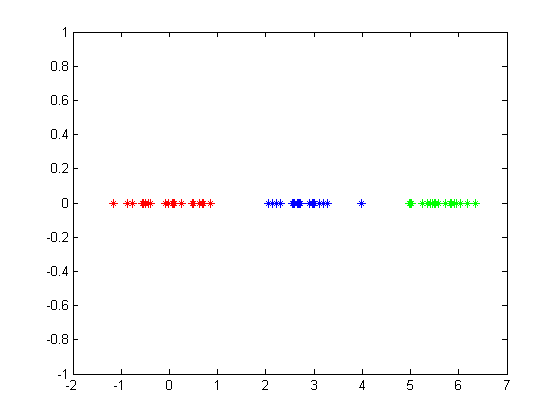
\includegraphics[width=120mm]{img/tp4/ej2-3.png}
\caption{Conjuntos de datos proyectados en $W$(vector).}
\end{figure}

\subsection{Ejercicio 3}

Aplicación de los programas desarrollados en los dos puntos anteriores a datos Gaussianos multidimensionales
isotrópicos.

\subsubsection{Resultados e Imágenes, 2 Clases}

Clase 1 (Azul): 45 elementos, $\mu$ = [1;1], $\sigma$ = [0.25 0 ; 0 0.25]\\
Clase 2 (Verde): 45 elementos, $\mu$ = [-1;-1], $\sigma$ = [0.25 0 ; 0 0.25]\\

\begin{figure}[ht!]
\centering
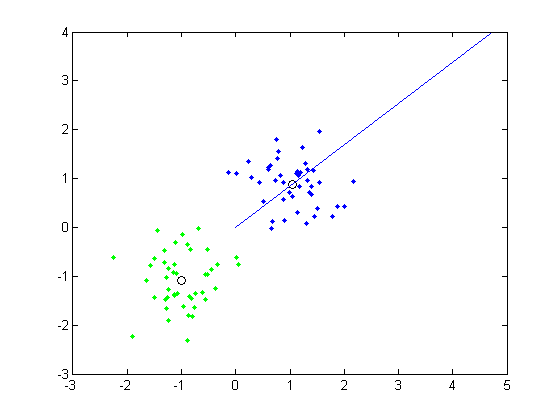
\includegraphics[width=120mm]{img/tp4/ej3-1.png}
\caption{Conjuntos de datos en dos dimensiónes y $W$.}
\end{figure}

\begin{figure}[ht!]
\centering
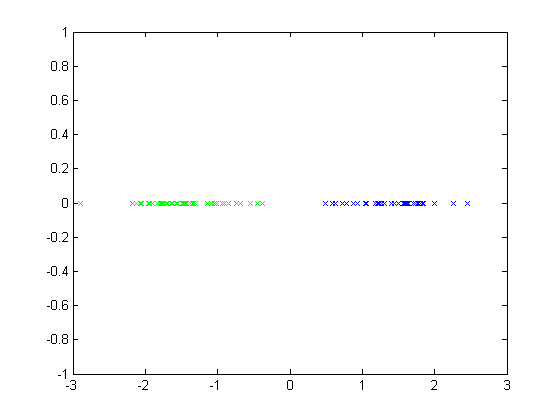
\includegraphics[width=120mm]{img/tp4/ej3-2.png}
\caption{Conjuntos de datos ya proyectados en $W$.}
\end{figure}

\subsubsection{Resultados e Imágenes, 3 Clases}

Clase 1 (Rojo): 45 elementos, $\mu$ = [0;0;0], $\sigma$ = [0.25 0 0 ; 0 0.25 0 ; 0 0 0.25]\\
Clase 2 (Azul): 45 elementos, $\mu$ = [2;2;2], $\sigma$ = [0.25 0 0 ; 0 0.25 0 ; 0 0 0.25]\\
Clase 3 (Verde): 45 elementos, $\mu$ = [1;4;4], $\sigma$ = [0.25 0 0 ; 0 0.25 0 ; 0 0 0.25]

\begin{figure}[ht!]
\centering
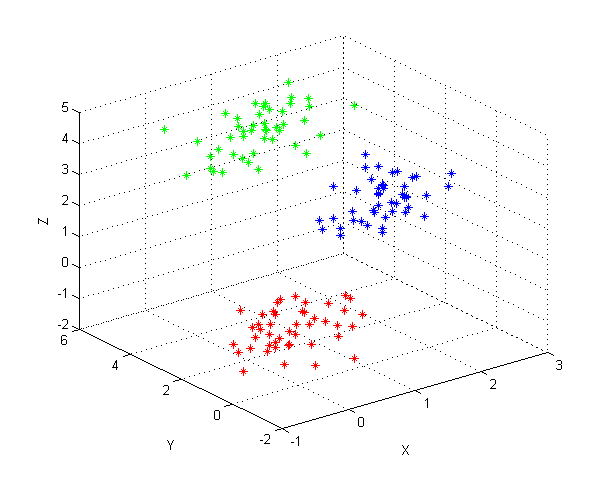
\includegraphics[width=120mm]{img/tp4/ej3-3.png}
\caption{Conjuntos de datos en tres dimensiónes.}
\end{figure}

\begin{figure}[ht!]
\centering
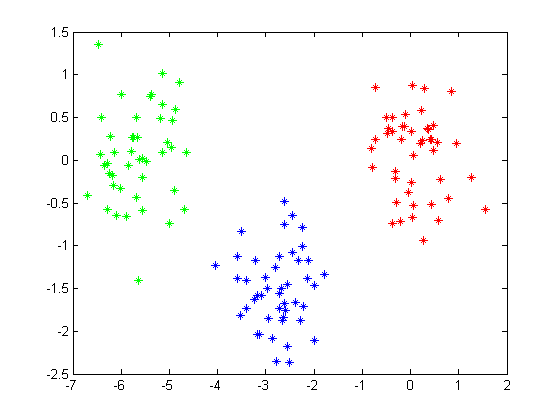
\includegraphics[width=120mm]{img/tp4/ej3-4.png}
\caption{Conjuntos de datos ya proyectados en $W$(plano).}
\end{figure}

\begin{figure}[ht!]
\centering
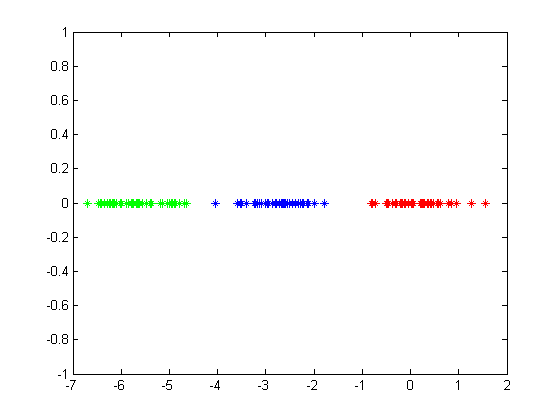
\includegraphics[width=120mm]{img/tp4/ej3-5.png}
\caption{Conjuntos de datos ya proyectados en $W$(vector).}
\end{figure}

\subsection{Ejercicio 4}

Luego de probar varios grados de separacion llegamos a la conclusion de que existen tres casos significativos.\\
Utilizamos dos clases con a datos Gaussianos multidimensionales
isotrópicos. Una clase fija, de 45 elementos, $\mu$ = [0;0] y $\sigma$ = [0.25 0 ; 0 0.25] y una segunda clase que varia en cada caso.

\subsubsection{Resultados e Imágenes}

El primer caso es el optimo, en el cual ambas clases tienen medias muy distantes y los datos en ningun momento se mezclan. Esto permite que el discriminante lineal de Fisher retorne un resultado muy facil de clasificar.\\
Segunda clase: $\mu$ = [2;2] y $\sigma$ = [0.25 0 ; 0 0.25]

\begin{figure}[ht!]
\centering
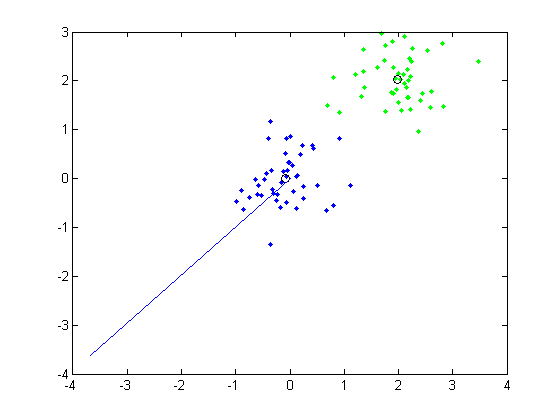
\includegraphics[width=120mm]{img/tp4/ej4-1.png}
\caption{Conjuntos de datos en dos dimensiónes y $W$.}
\end{figure}

\begin{figure}[ht!]
\centering
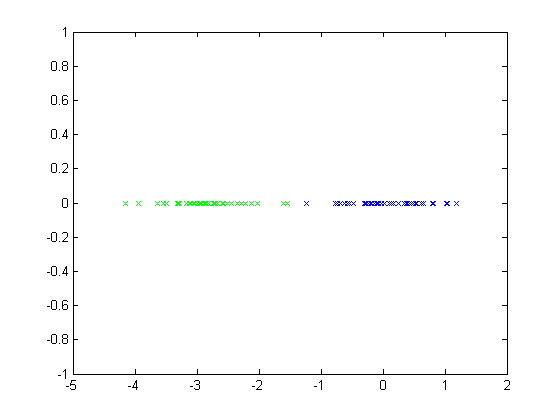
\includegraphics[width=120mm]{img/tp4/ej4-2.png}
\caption{Conjuntos de datos ya proyectados en $W$.}
\end{figure}

El segundo es aquel en el cual las medias son cercanas y algunos de sus elementos se mezclan. Esto hace que el discriminante lineal de Fisher retorne un resultado que al clasificarlo no es perfecto, pero se aproxima bastante.\\
Segunda clase: $\mu$ = [0.7;0.7] y $\sigma$ = [0.25 0 ; 0 0.25]

\begin{figure}[ht!]
\centering
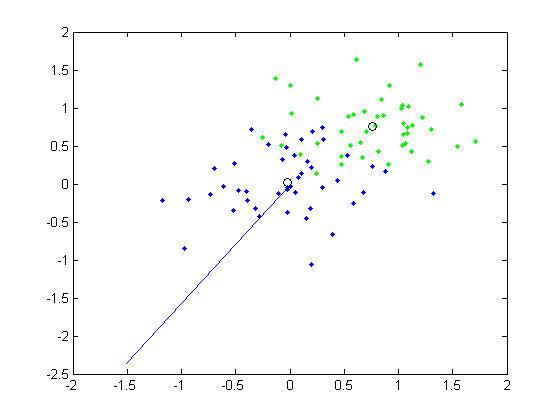
\includegraphics[width=120mm]{img/tp4/ej4-3.png}
\caption{Conjuntos de datos en dos dimensiónes y $W$.}
\end{figure}

\begin{figure}[ht!]
\centering
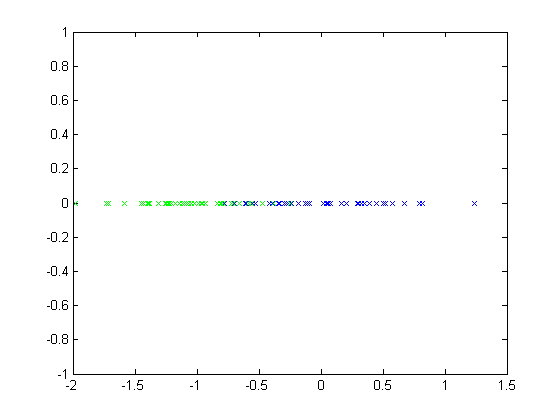
\includegraphics[width=120mm]{img/tp4/ej4-4.png}
\caption{Conjuntos de datos ya proyectados en $W$.}
\end{figure}

El tercero es aquel en el cual las medias son muy similares o iguales y la mayoria de elementos se mezclan. Esto hace que el discriminante lineal de Fisher retorne un resultado imposible de clasificar. Este metodo no es eficaz para esta clase de datos.\\
Segunda clase: $\mu$ = [0;0] y $\sigma$ = [0.25 0 ; 0 0.25]

\begin{figure}[ht!]
\centering
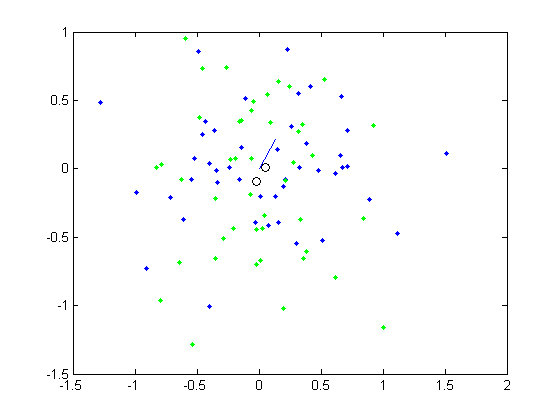
\includegraphics[width=120mm]{img/tp4/ej4-5.png}
\caption{Conjuntos de datos en dos dimensiónes y $W$.}
\end{figure}

\begin{figure}[ht!]
\centering
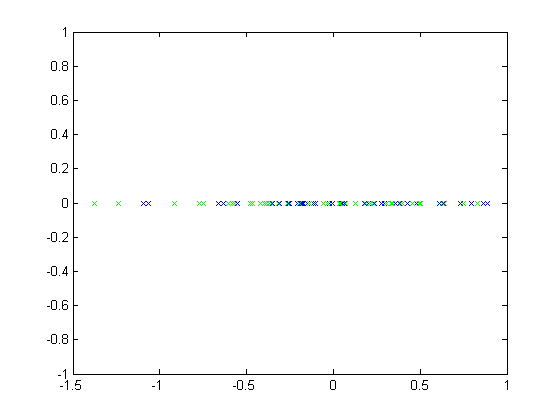
\includegraphics[width=120mm]{img/tp4/ej4-6.png}
\caption{Conjuntos de datos ya proyectados en $W$.}
\end{figure}

\newpage

\section{TP5: Expectation Maximization}
\input{tp5.tex}
\newpage

\end{document}
